  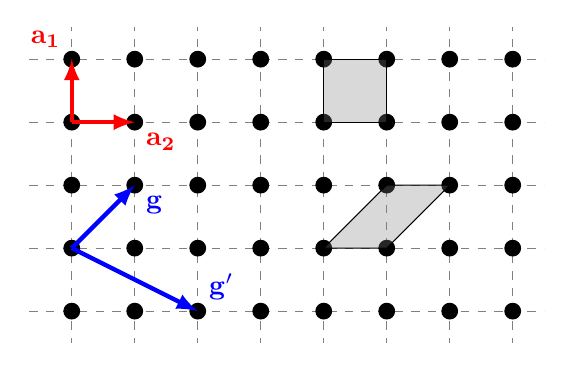
\begin{tikzpicture}[scale=0.80]
    \coordinate (Origin)   at (-7,-4);
    \coordinate (XAxisMin) at (-3,0);
    \coordinate (XAxisMax) at (3,0);
    \coordinate (YAxisMin) at (0,-3);
    \coordinate (YAxisMax) at (0,3);
%    \draw [thin, gray,-latex] (XAxisMin) -- (XAxisMax);% Draw x axis
%    \draw [thin, gray,-latex] (YAxisMin) -- (YAxisMax);% Draw y axis

    \clip (-7.7,-0.5) rectangle (0.5,4.5); % Clips the picture...
    %\pgftransformcm{1}{0.0}{0.0}{1}{\pgfpoint{0cm}{0cm}}
          % This is actually the transformation matrix entries that
          % gives the slanted unit vectors. You might check it on
           % MATLAB etc. . I got it by guessing.
    \coordinate (Bone) at (0,1);
    \coordinate (Btwo) at (2,-2);
    \draw[style=help lines,dashed] (-14,-14) grid[step=1cm] (14,14);
          % Draws a grid in the new coordinates.
          %\filldraw[fill=gray, fill opacity=0.3, draw=black] (0,0) rectangle (2,2);
              % Puts the shaded rectangle
    \foreach \x in {-7,...,7}{% Two indices running over each
      \foreach \y in {-4,-3,...,4}{% node on the grid we have drawn 
        \node[draw,circle,inner sep=2pt,fill] at (\x,\y) {};
            % Places a dot at those points
      }
    }
    \draw [ultra thick,-latex,red] (-7,3)
        -- +(0,1) node [above left] {$\mathbf{a_1}$};
    \draw [ultra thick,-latex,red] (-7,3)
        -- +(1,0) node [below right] {$\mathbf{a_2}$};
    \draw [ultra thick,-latex,blue] (-7,1)
        -- (-6,2) node [below right] {$\mathbf{g}$};
    \draw [ultra thick,-latex,blue] (-7,1)
        -- (-5,0) node [above right] {$\mathbf{g'}$};
	    
    \filldraw[fill=gray, fill opacity=0.3, draw=black] (-3,3)
        rectangle (-2,4);
    \filldraw[fill=gray, fill opacity=0.3, draw=black] (-3,1)
        -- (-2,1) -- (-1,2) -- (-2,2) -- cycle;
    %\draw [thin,-latex,red, fill=gray, fill opacity=0.3] (0,0)
        % -- ($2*(0,2)+(2,-2)$)
        % -- ($3*(0,2)+2*(2,-2)$) -- ($(0,2)+(2,-2)$) -- cycle;
  \end{tikzpicture}
  \caption{Espacio directo}
  %\caption{Malla cuadrada en el espacio directo. Los vectores $\mathbf{a_1}$ y $\mathbf{a_2}$ son unos de los posibles vectores base de la malla; los vectores $\mathbf{g}$, $\mathbf{g'}$ y $\mathbf{g'}$ son combinaciones lineales de éstos. Las zonas sombreadas son  celdas unitarias. }
  \label{malla1}